\documentclass[12pt, oneside]{article}

\usepackage[letterpaper, scale=0.89, centering]{geometry}
\usepackage{fancyhdr}
\setlength{\parindent}{0em}
\setlength{\parskip}{1em}

\usepackage{tikz}
\usetikzlibrary{automata,positioning,arrows}

\pagestyle{fancy}
\fancyhf{}
\renewcommand{\headrulewidth}{0pt}
\rfoot{\href{https://creativecommons.org/licenses/by-nc-sa/2.0/}{CC BY-NC-SA 2.0} Version \today~(\thepage)}

\usepackage{amssymb,amsmath,pifont,amsfonts,comment,enumerate,enumitem}
\usepackage{currfile,xstring,hyperref,tabularx,graphicx,wasysym}
\usepackage[labelformat=empty]{caption}
\usepackage{xcolor}
\usepackage{multicol,multirow,array,listings,tabularx,lastpage,textcomp,booktabs}

\lstnewenvironment{algorithm}[1][] {   
    \lstset{ mathescape=true,
        frame=tB,
        numbers=left, 
        numberstyle=\tiny,
        basicstyle=\rmfamily\scriptsize, 
        keywordstyle=\color{black}\bfseries,
        keywords={,procedure, div, for, to, input, output, return, datatype, function, in, if, else, foreach, while, begin, end, }
        numbers=left,
        xleftmargin=.04\textwidth,
        #1
    }
}
{}

\newcommand\abs[1]{\lvert~#1~\rvert}
\newcommand{\st}{\mid}

\newcommand{\cmark}{\ding{51}}
\newcommand{\xmark}{\ding{55}}
 
\begin{document}
\begin{flushright}
    \StrBefore{\currfilename}{.}
\end{flushright} \section*{Week4 monday}


Recap so far: In DFA, the only memory available is in the states. Automata can only
``remember'' finitely far in the past and finitely much information, because
they can have only finitely many states. If a computation path of a DFA visits 
the same state more than once, the machine can't tell the difference between 
the first time and future times it visits this state. Thus, if 
a DFA accepts one long string, then it must accept (infinitely) many 
similar strings.

{\bf Definition}  A positive integer $p$ is a {\bf pumping length} of a language $L$ over $\Sigma$ means
that, for each string $s  \in  \Sigma^*$, if  $|s| \geq p$ and $s \in L$, then there are strings $x,y,z$
such that 
\[
s = xyz
\]
and  
\[
|y| > 0,  \qquad \qquad 
\text{ for each $i \geq 0$, $xy^i z \in L$}, \qquad \text{and}
\qquad  \qquad
|xy| \leq p.
\]

{\bf Negation}: A positive integer  $p$  is {\bf not a pumping length} of a language  $L$ over  $\Sigma$  iff
\[
\exists s \left(~  |s| \geq  p \wedge s \in L \wedge \forall x \forall y \forall z  \left( ~\left( s = xyz \wedge 
|y| > 0 \wedge |xy| \leq p~ \right) \to \exists i  (  i \geq 0  \wedge xy^iz  \notin L ) \right) ~\right) 
\]
{\it Informally: }


Restating {\bf Pumping Lemma}: If $L$ is a regular language, then it  has
a pumping length.


{\bf Contrapositive}: If $L$ has no pumping length, then  it is nonregular.

\vfill

{\Large The Pumping Lemma {\it cannot} be used to prove that a language {\it is} regular.} 

{\Large The Pumping Lemma {\bf can} be used to prove that a language {\it is not} regular.}

{\it Extra practice}: Exercise 1.49 in the book.


\vfill

{\bf Proof strategy}: To prove that a language $L$ is {\bf not} regular, 
\begin{itemize}
    \item Consider an arbitrary positive integer $p$
    \item Prove that $p$ is not a pumping length for $L$
    \item Conclude that $L$ does not have {\it any} pumping length, and therefore it is not regular.
\end{itemize}

\newpage
{\bf Example}: $\Sigma  =  \{0,1\}$, $L = \{ 0^n 1^n \mid n  \geq 0\}$.

Fix $p$ an arbitrary positive integer. List strings that are in $L$ and have length  greater than or equal  to $p$:

\vspace{20pt}

Pick $s = $


Suppose $s = xyz$ with  $|xy|  \leq  p$ and $|y| > 0$.
\begin{center}
\begin{tabular}{|c|}
\hline
 \\
\hspace{4in} \\
\hline
\end{tabular}
\end{center}

Then when $i = \hspace{1in}$, $xy^i z  = \hspace{1in}$

\newpage

{\bf Example}: $\Sigma  =  \{0,1\}$, $L = \{w w^{\mathcal{R}} \mid w \in \{0,1\}^*\}$.
Remember that the reverse of a string $w$ is denoted $w^\mathcal{R}$  
and means to write $w$  in  the opposite order, if $w = w_1 \cdots  w_n$ then $w^\mathcal{R} = w_n \cdots  w_1$. Note: $\varepsilon^\mathcal{R} = \varepsilon$.


Fix $p$ an arbitrary positive integer. List strings that are in $L$ and have length  greater than or equal  to $p$:

\vspace{10pt}

Pick $s = $

Suppose $s = xyz$ with  $|xy|  \leq  p$ and $|y| > 0$.
\begin{center}
\begin{tabular}{|c|}
\hline
 \\
\hspace{4in} \\
\hline
\end{tabular}
\end{center}
Then when $i = \hspace{1in}$, $xy^i z  = \hspace{1in}$


\vspace{30pt} 

{\bf Example}: $\Sigma  =  \{0,1\}$, $L = \{0^j1^k  \mid j \geq k  \geq 0\}$.

Fix $p$ an arbitrary positive integer. List strings that are in $L$ and have length  greater than or equal  to $p$:

\vspace{10pt}

Pick $s = $


Suppose $s = xyz$ with  $|xy|  \leq  p$ and $|y| > 0$.
\begin{center}
\begin{tabular}{|c|}
\hline
 \\
\hspace{4in} \\
\hline
\end{tabular}
\end{center}
Then when $i = \hspace{1in}$, $xy^i z  = \hspace{1in}$



\vspace{30pt} 

{\bf Example}: $\Sigma  =  \{0,1\}$, $L = \{0^n1^m0^n  \mid m,n  \geq 0\}$.

Fix $p$ an arbitrary positive integer. List strings that are in $L$ and have length  greater than or equal  to $p$:

\vspace{10pt}

Pick $s = $


Suppose $s = xyz$ with  $|xy|  \leq  p$ and $|y| > 0$.
\begin{center}
\begin{tabular}{|c|}
\hline
 \\
\hspace{4in} \\
\hline
\end{tabular}
\end{center}
Then when $i = \hspace{1in}$, $xy^i z  = \hspace{1in}$

\newpage
{\it Extra practice}:


\begin{center}
    \begin{tabular}{c|c| c| c}
    Language & $s \in L$ & $s \notin L$ & Is the language regular or nonregular?  \\
    \hline
     & \hspace{1in} & \hspace{1in}  &  \\
    $\{a^nb^n \mid 0  \leq n  \leq 5 \}$ & & & \\
     & & & \\
    $\{b^n a^n \mid  n  \geq 2\}$  & & & \\
     & & & \\
    $\{a^m b^n \mid  0 \leq m\leq n\}$  & & & \\
     & & & \\
    $\{a^m b^n \mid  m \geq n+3,  n \geq 0\}$  & & & \\
     & & & \\
    $\{b^m a^n \mid  m \geq 1, n \geq  3\}$  & & & \\
     & & & \\
    $\{ w  \in \{a,b\}^* \mid w = w^\mathcal{R} \}$ & & & \\
     & & & \\ 
    $\{ ww^\mathcal{R} \mid w\in \{a,b\}^* \}$ & & & \\
     & & & \\ 
    \end{tabular}
\end{center}
     \vfill
\section*{Week4 wednesday}


Regular sets are not the end of the story
\begin{itemize}
    \item Many nice / simple / important sets are not regular
    \item Limitation of the finite-state automaton model: Can't ``count", Can only remember finitely far into the past,
    Can't backtrack, Must make decisions in ``real-time"
    \item We know actual computers are more powerful than this model...
\end{itemize}

The {\bf next} model of computation. Idea: allow some memory of unbounded size. How? 
\begin{itemize}
    \item To generalize regular expressions: {\bf context-free grammars}\\
    \item To generalize NFA: {\bf Pushdown automata}, which is like an NFA with access to a stack: 
    Number of states is fixed, number of entries in stack is unbounded. At each step
    (1) Transition to new state based on current state, letter read, and top letter of stack, then
    (2) (Possibly) push or pop a letter to (or from) top of stack. Accept a string iff
    there is some sequence of states and some sequence of stack contents 
    which helps the PDA processes the entire input string and ends in an accepting state.
\end{itemize}

\vfill

\vfill

Is there a PDA that recognizes the nonregular language $\{0^n1^n \mid n \geq 0 \}$?

\vfill

\newpage


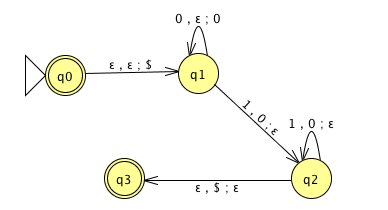
\includegraphics[width=4in]{../../resources/machines/Lect9PDA.png}

The PDA with state diagram above can be informally described as:
\begin{quote}
    Read symbols from the input. As each 0 is read, push it onto the stack. 
    As soon as 1s are seen, pop a 0 off the stack for each 1 read. 
    If the stack becomes empty and we are at the end of the input string, accept the input. 
    If the stack becomes empty and there are 1s left to read, 
    or if 1s are finished while the stack still contains 0s, or if any 0s
    appear in the string following 1s, 
    reject the input.
\end{quote}
    

Trace the computation of this PDA on the input string $01$.

\vfill
    
Trace the computation of this PDA on the input string $011$.

\vfill

\newpage
A PDA recognizing the set $\{ \hspace{1.5 in} \}$ can be informally described as:
\begin{quote}
    Read symbols from the input. As each 0 is read, push it onto the stack. 
    As soon as 1s are seen, pop a 0 off the stack for each 1 read. 
    If the stack becomes empty and there is exactly one 1 left to read, read that 1 and accept the input. 
    If the stack becomes empty and there are either zero or more than one 1s left to read, 
    or if the 1s are finished while the stack still contains 0s, or if any 0s appear in the input following 1s, 
    reject the input.
\end{quote}
Modify the state diagram below to get a PDA that implements this description:

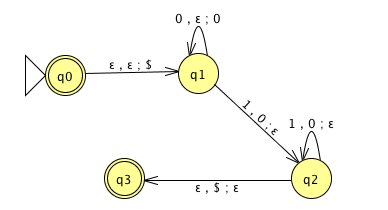
\includegraphics[width=4in]{../../resources/machines/Lect9PDA.png}


\vfill
{\bf Definition} A {\bf pushdown automaton} (PDA) is  specified by a  $6$-tuple $(Q, \Sigma, \Gamma, \delta, q_0, F)$
where $Q$ is the finite set of states, $\Sigma$ is the input alphabet,  $\Gamma$ is the stack alphabet,
\[
    \delta: Q \times \Sigma_\varepsilon  \times  \Gamma_\varepsilon \to \mathcal{P}( Q \times \Gamma_\varepsilon)
\]
is the transition function,  $q_0 \in Q$ is the start state, $F \subseteq  Q$ is the set of accept states.
    
 \vfill
\section*{Week4 friday}




Draw the state diagram and give the formal definition of a PDA with $\Sigma = \Gamma$.

\vfill

Draw the state diagram and give the formal definition of a PDA with $\Sigma \cap \Gamma = \emptyset$.
    
\vfill

\newpage
For the PDA state diagrams below, $\Sigma = \{0,1\}$.


\begin{center}
\begin{tabular}{c c}
Mathematical description of language & State diagram of PDA recognizing language\\
\hline
& $\Gamma = \{ \$, \#\}$ \hspace{2.3in} \\
& \\
& 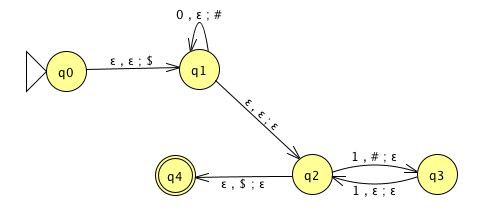
\includegraphics[width=3.5in]{../../resources/machines/Lect10PDA1.png}\\
& \\
& \\
\hline
& $\Gamma = \{ {@}, 1\}$ \hspace{2.3in} \\
& \\
& 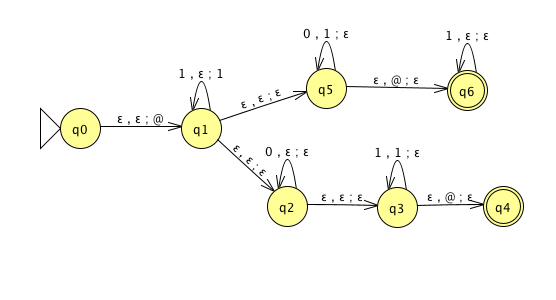
\includegraphics[width=3.5in]{../../resources/machines/Lect10PDA2.png}\\
& \\
& \\
\hline
& \\
& \\
& \\
$\{ 0^i 1^j 0^k \mid i,j,k \geq 0 \}$ & \\
& \\
& \\
\end{tabular}
\end{center}

 \vfill
 {\it Note: alternate notation is to replace $;$ with $\to$}

\begin{comment}
{\it Extra practice}: Consider the state diagram of a PDA with input alphabet 
$\Sigma$ and stack alphabet $\Gamma$.

\begin{center}
\begin{tabular}{|c|c|}
\hline
Label & means \\
\hline
$a, b ; c$ when $a \in \Sigma$, $b\in \Gamma$, $c \in \Gamma$ 
& \hspace{3in} \\
& \\
& \\
& \\
& \\
&\\
\hline
$a, \varepsilon ; c$ when $a \in \Sigma$, $c \in \Gamma$ 
& \hspace{3in} \\
& \\
& \\
& \\
& \\
&\\
\hline
$a, b ; \varepsilon$ when $a \in \Sigma$, $b\in \Gamma$
& \hspace{3in} \\
& \\
& \\
& \\
& \\
&\\
\hline
$a, \varepsilon ; \varepsilon$ when $a \in \Sigma$
& \hspace{3in} \\
& \\
& \\
& \\
& \\
&\\
\hline
\end{tabular}
\end{center}


How does the meaning change if $a$ is replaced by $\varepsilon$?
\end{comment}


{\it Big picture}: PDAs were motivated by wanting to add some memory of unbounded size to NFA. How 
do we accomplish a similar enhancement of regular expressions to get a syntactic model that is 
more expressive?

DFA, NFA, PDA: Machines process one input string at a time; the computation of a machine on its input string 
reads the input from left to right.

Regular expressions: Syntactic descriptions of all strings that match a particular pattern; the language 
described by a regular expression is built up recursively according to the expression's syntax

{\bf Context-free grammars}: Rules to produce one string at a time, adding characters from the middle, beginning, 
or end of the final string as the derivation proceeds.

 \vfill
\section*{Week3 monday}


{\bf Warmup}: Design a DFA (deterministic finite automaton) and an NFA (nondeterministic
finite automaton) that each recognize each of the following languages over $\{a,b\}$
\[
    \{ w \mid \text{$w$ has an $a$ and ends in $b$}\}
\]

\vfill

\[
    \{ w \mid \text{$w$ has an $a$ or ends in $b$}\}
\]

\vfill



\textbf{Strategy}: To design DFA or NFA for a given language,  
identify patterns that can be built up as we process strings and create states
for intermediate stages. Or: decompose the language to a simpler one 
that we already know how to recognize with a DFA or NFA.


{\it Recall} (from Wednesday of last week, and in textbook Exercise 1.14): 
if there is a DFA $M$ such that $L(M) = A$ then there is another DFA, let's call it $M'$, such that 
$L(M') = \overline{A}$, the complement of $A$, defined as $\{ w \in \Sigma^* \mid w \notin A \}$.


Let's practice defining automata constructions by coming up with other ways to get new automata from old.
\newpage

Suppose $A_1, A_2$ are languages over an alphabet $\Sigma$.
{\bf Claim:} if there is a NFA $N_1$ such that $L(N_1) = A_1$ and 
NFA $N_2$ such that $L(N_2) = A_2$, then there is another NFA, let's call it $N$, such that 
$L(N) = A_1 \cup A_2$.

{\bf Proof idea}: Use nondeterminism to choose which of $N_1$, $N_2$ to run.

\vfill
\begin{comment}
    Draw schematic
\end{comment}

{\bf Formal construction}: Let 
$N_1 = (Q_1, \Sigma, \delta_1, q_1, F_1)$ and $N_2 = (Q_2, \Sigma, \delta_2,q_2, F_2)$
and assume $Q_1 \cap Q_2 = \emptyset$ and that $q_0 \notin Q_1 \cup Q_2$.
Construct $N = (Q, \Sigma, \delta, q_0, F_1 \cup F_2)$ where
\begin{itemize}
    \item $Q = $
    \item $\delta: Q \times \Sigma_\varepsilon \to \mathcal{P}(Q)$ is defined by, for $q \in Q$ and $x \in \Sigma_{\varepsilon}$:
        \[
            \phantom{\delta((q,x))=\begin{cases}  \delta_1 ((q,x)) &\qquad\text{if } q\in Q_1 \\ \delta_2 ((q,x)) &\qquad\text{if } q\in Q_2 \\ \{q1,q2\} &\qquad\text{if } q = q_0, x = \varepsilon \\ \emptyset\text{if } q= q_0, x \neq \varepsilon \end{cases}}
        \]
\end{itemize}


\vfill
{\it Proof of correctness would prove that $L(N) = A_1 \cup A_2$ by considering
an arbitrary string accepted by $N$, tracing an accepting computation of $N$ on it, and using 
that trace to prove the string is in at least one of $A_1$, $A_2$; then, taking an arbitrary 
string in $A_1 \cup A_2$ and proving that it is accepted by $N$. Details left for extra practice.}


{\bf Example}: The language recognized by the NFA over $\{a,b\}$ with state diagram


    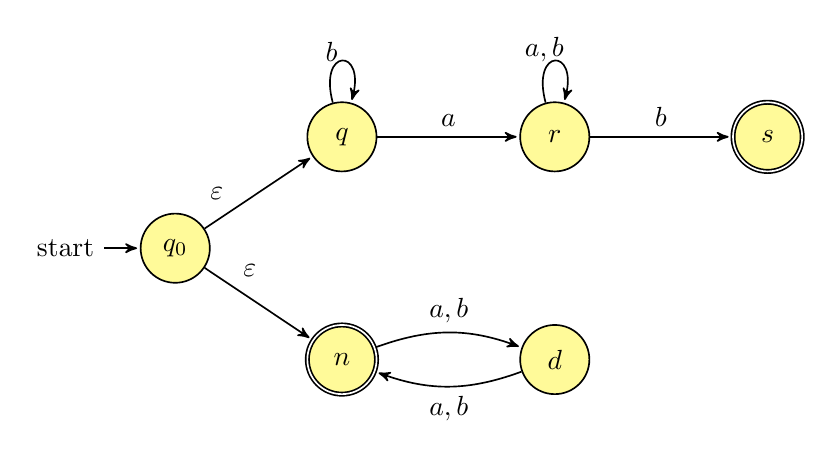
\begin{tikzpicture}[->,>=stealth',shorten >=1pt, auto, node distance=2cm, semithick]
    \tikzstyle{every state}=[text=black, fill=yellow!40]
    
    \node[initial,state] (q0)          {$q_0$};
    \node[state]         (q) [above right of=q0, xshift=20pt] {$q$};
    \node[state]         (r) [right of=q, xshift=20pt] {$r$};
    \node[state, accepting]         (s) [right of=r, xshift=20pt] {$s$};
    \node[state, accepting]         (n) [below right of=q0, xshift=20pt] {$n$};
    \node[state]         (d) [right of=n, xshift=20pt] {$d$};
    
    \path (q0) edge  [bend left=0, near start] node {$\varepsilon$} (q)
            edge [bend right=0, near start] node {$\varepsilon$} (n)
        (q) edge [bend left=0] node {$a$} (r)
            edge [loop above, near start] node {$b$} (q)
        (r) edge [bend left=0] node {$b$} (s)
            edge [loop above, near start] node {$a,b$} (r)
        (n) edge [bend left=20] node {$a,b$} (d)
        (d) edge [bend left=20] node {$a,b$} (n)
    ;
    \end{tikzpicture}
is:


\newpage

Could we do the same construction with DFA?

\vspace{50pt}

Happily, though, an analogous claim is true!

Suppose $A_1, A_2$ are languages over an alphabet $\Sigma$.
{\bf Claim:} if there is a DFA $M_1$ such that $L(M_1) = A_1$ and 
DFA $M_2$ such that $L(M_2) = A_2$, then there is another DFA, let's call it $M$, such that 
$L(M) = A_1 \cup A_2$. {\it Theorem 1.25 in Sipser, page 45}
    
    {\bf Proof idea}:
    
    
    {\bf Formal construction}: 
    
    \vfill

    
    {\bf Example}:  When $A_1 = \{w \mid w~\text{has an $a$ and ends in $b$} \}$ and 
    $A_2 = \{ w \mid w~\text{is of even length} \}$.
    
    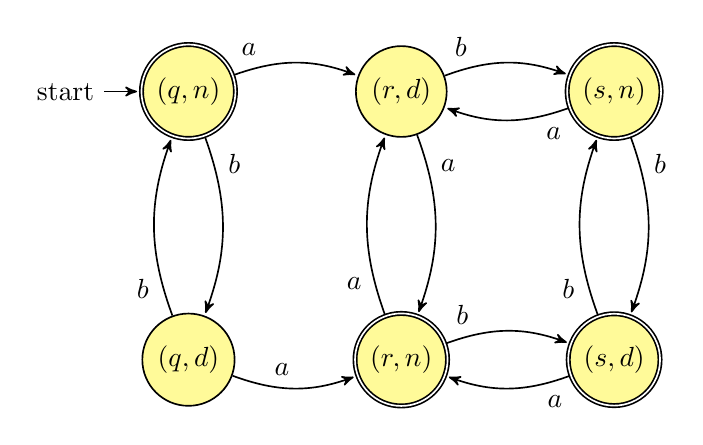
\begin{tikzpicture}[->,>=stealth',shorten >=1pt, auto, node distance=2cm, semithick]
        \tikzstyle{every state}=[text=black, fill=yellow!40]
        
        \node[initial,state,accepting] (qn)          {$(q,n)$};
        \node[state]         (qd) [below of=qn, yshift=-40pt] {$(q,d)$};
        \node[state]         (rd) [right of=qn, xshift=20pt] {$(r,d)$};
        \node[state,accepting]         (rn) [right of=qd, xshift=20pt] {$(r,n)$};
        \node[state,accepting]         (sn) [right of=rd, xshift=20pt] {$(s,n)$};
        \node[state,accepting]         (sd) [right of=rn, xshift=20pt] {$(s,d)$};
        
        \path (qn) edge  [bend left=20, near start] node {$b$} (qd)
                edge [bend left=20, near start] node {$a$} (rd)
            (qd) edge [bend left=20, near start] node {$b$} (qn)
                edge [bend right=20, near start] node {$a$} (rn)
            (rn) edge [bend left=20, near start] node {$a$} (rd)
                edge [bend left=20, near start] node {$b$} (sd)
            (rd) edge [bend left=20, near start] node {$a$} (rn)
                edge [bend left=20, near start] node {$b$} (sn)
            (sn) edge [bend left=20, near start] node {$a$} (rd)
                edge [bend left=20, near start] node {$b$} (sd)
            (sd) edge [bend left=20, near start] node {$a$} (rn)
                edge [bend left=20, near start] node {$b$} (sn)
        ;
        \end{tikzpicture}
    
    \newpage
    
    Suppose $A_1, A_2$ are languages over an alphabet $\Sigma$.
    {\bf Claim:} if there is a DFA $M_1$ such that $L(M_1) = A_1$ and 
    DFA $M_2$ such that $L(M_2) = A_2$, then there is another DFA, let's call it $M$, such that 
    $L(M) = A_1 \cap A_2$.  {\it Sipser Theorem 1.25, page 45}
    
    {\bf Proof idea}:
    
    
    {\bf Formal construction}: 
    
    \vspace{70pt}


    
    

 \vfill
\section*{Week3 wednesday}


So far we have that: 
\begin{itemize}
\item If there is a DFA recognizing a language, there is a DFA recognizing its complement.
\item If there are NFA recognizing two languages, there is a NFA recognizing their union.
\item If there are DFA recognizing two languages, there is a DFA recognizing their union.
\item If there are DFA recognizing two languages, there is a DFA recognizing their intersection.
\end{itemize}

Our goals for today are (1) prove similar results about other set operations, (2) prove that 
NFA and DFA are equally expressive, and therefore (3) define an important class of languages.

\vfill

Suppose $A_1, A_2$ are languages over an alphabet $\Sigma$.
{\bf Claim:} if there is a NFA $N_1$ such that $L(N_1) = A_1$ and 
NFA $N_2$ such that $L(N_2) = A_2$, then there is another NFA, let's call it $N$, such that 
$L(N) = A_1 \circ A_2$.

{\bf Proof idea}: Allow computation to move between $N_1$ and $N_2$ ``spontaneously" when reach an accepting state of 
$N_1$, guessing that we've reached the point where the two parts of the string in the set-wise concatenation 
are glued together.


{\bf Formal construction}: Let 
$N_1 = (Q_1, \Sigma, \delta_1, q_1, F_1)$ and $N_2 = (Q_2, \Sigma, \delta_2,q_2, F_2)$
and assume $Q_1 \cap Q_2 = \emptyset$.
Construct $N = (Q, \Sigma, \delta, q_0, F)$ where
\begin{itemize}
    \item $Q = $
    \item $q_0 = $
    \item $F = $
    \item $\delta: Q \times \Sigma_\varepsilon \to \mathcal{P}(Q)$ is defined by, for $q \in Q$ and $a \in \Sigma_{\varepsilon}$:
        \[
            \delta((q,a))=\begin{cases}  
                \delta_1 ((q,a)) &\qquad\text{if } q\in Q_1 \textrm{ and } q \notin F_1\\ 
                \delta_1 ((q,a)) &\qquad\text{if } q\in F_1 \textrm{ and } a \in \Sigma\\ 
                \delta_1 ((q,a)) \cup \{q_2\} &\qquad\text{if } q\in F_1 \textrm{ and } a = \varepsilon\\ 
                \delta_2 ((q,a)) &\qquad\text{if } q\in Q_2
            \end{cases}
        \]
\end{itemize}

\vfill

{\it Proof of correctness would prove that $L(N) = A_1 \circ A_2$ by considering
an arbitrary string accepted by $N$, tracing an accepting computation of $N$ on it, and using 
that trace to prove the string can be written as the result of concatenating two strings, 
the first in $A_1$ and the second in $A_2$; then, taking an arbitrary 
string in $A_1 \circ A_2$ and proving that it is accepted by $N$. Details left for extra practice.}

\newpage



Suppose $A$ is a language over an alphabet $\Sigma$.
{\bf Claim:} if there is a NFA $N$ such that $L(N) = A$, then there is another NFA, let's call it $N'$, such that 
$L(N') = A^*$.

{\bf Proof idea}: Add a fresh start state, which is an accept state. Add spontaneous 
moves from each (old) accept state to the old start state.

{\bf Formal construction}: Let 
$N = (Q, \Sigma, \delta, q_1, F)$ and assume $q_0 \notin Q$.
Construct $N' = (Q', \Sigma, \delta', q_0, F')$ where
\begin{itemize}
    \item $Q' = Q \cup \{q_0\}$
    \item $F' = F \cup \{q_0\}$
    \item $\delta': Q' \times \Sigma_\varepsilon \to \mathcal{P}(Q')$ is defined by, for $q \in Q'$ and $a \in \Sigma_{\varepsilon}$:
        \[
            \delta'((q,a))=\begin{cases}  
                \delta ((q,a)) &\qquad\text{if } q\in Q \textrm{ and } q \notin F\\ 
                \delta ((q,a)) &\qquad\text{if } q\in F \textrm{ and } a \in \Sigma\\ 
                \delta ((q,a)) \cup \{q_1\} &\qquad\text{if } q\in F \textrm{ and } a = \varepsilon\\ 
                \{q_1\} &\qquad\text{if } q = q_0 \textrm{ and } a = \varepsilon \\
                \emptyset &\qquad\text{if } q = q_0 \textrm { and } a \in \Sigma
            \end{cases}
        \]
\end{itemize}


{\it Proof of correctness would prove that $L(N') = A^*$ by considering
an arbitrary string accepted by $N'$, tracing an accepting computation of $N'$ on it, and using 
that trace to prove the string can be written as the result of concatenating some number of strings, 
each of which is in $A$; then, taking an arbitrary 
string in $A^*$ and proving that it is accepted by $N'$. Details left for extra practice.}


{\bf Application}: A state diagram for a NFA over $\Sigma = \{a,b\}$ 
that recognizes $L (( a^*b)^* )$:

\vfill
\newpage
Suppose $A$ is a language over an alphabet $\Sigma$.
{\bf Claim:} if there is a NFA $N$ such that $L(N) = A$ then 
there is a DFA $M$ such that $L(M) = A$.

{\bf Proof idea}: States in $M$ are ``macro-states" -- collections of states from $N$ -- 
that represent the set of possible states a computation of $N$ might be in.


{\bf Formal construction}: Let $N = (Q, \Sigma, \delta, q_0, F)$.  Define 
\[
M = (~ \mathcal{P}(Q), \Sigma, \delta', q',  \{ X \subseteq Q \mid X \cap F \neq \emptyset \}~ )
\]
where $q' = \{ q \in Q \mid \text{$q = q_0$ or is accessible from $q_0$ by spontaneous moves in $N$} \}$
and 
\[
    \delta' (~(X, x)~) = \{ q \in Q \mid q \in \delta( ~(r,x)~) ~\text{for some $r \in X$ or is accessible 
from such an $r$ by spontaneous moves in $N$} \}
\]


Consider the state diagram of an NFA over $\{a,b\}$. Use the ``macro-state'' construction 
to find an equivalent DFA.

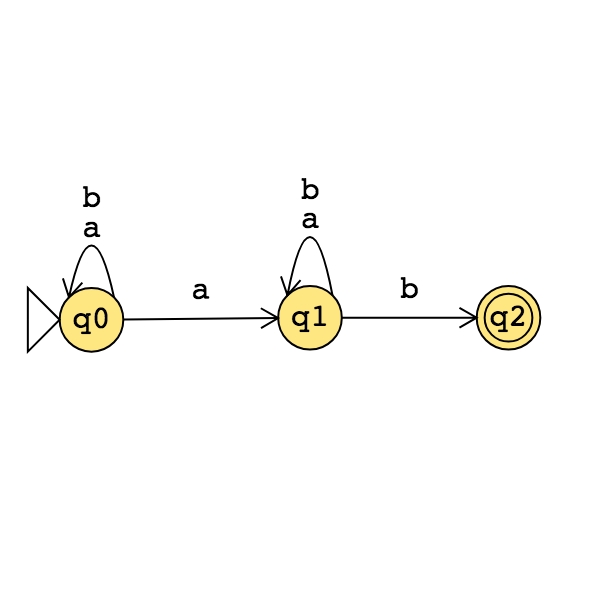
\includegraphics[width=2.5in]{../../resources/machines/Lect6NFA1.png}




\vfill

Consider the state diagram of an NFA over $\{0,1\}$. Use the ``macro-state'' construction 
to find an equivalent DFA.


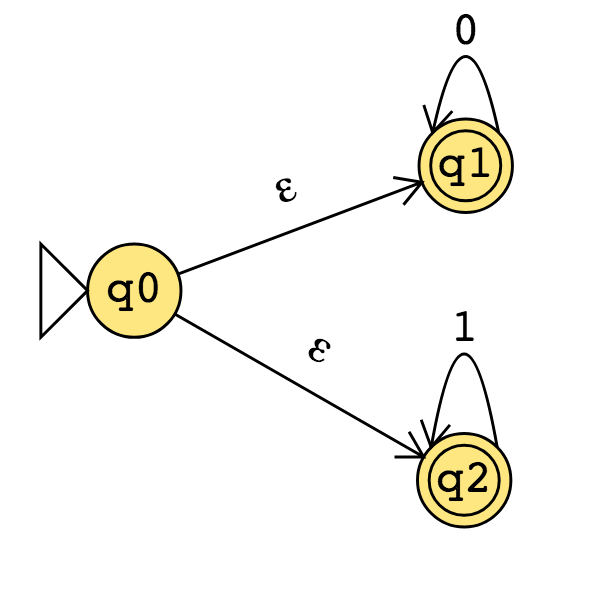
\includegraphics[width=1.8in]{../../resources/machines/Lect6NFA2.png}


\vfill

Note: We can often prune the DFAs that result from the ``macro-state'' constructions to get an 
equivalent DFA with fewer states (e.g.\ only the ``macro-states" reachable from the start state).

\newpage


{\bf The class of regular languages}

Fix an alphabet $\Sigma$. For each language $L$ over $\Sigma$:
\begin{center}
\begin{tabular}{cc}
    {\bf There is a DFA over $\Sigma$ that recognizes $L$}&$\exists M ~(M \textrm{ is a DFA and } L(M) = A)$\\
    {\it if and only if}&\\
    {\bf There is a NFA over $\Sigma$ that recognizes $L$}&$\exists N ~(N \textrm{ is a NFA and } L(N) = A)$\\
    {\it if and only if}&\\
    {\bf There is a regular expression over $\Sigma$ that describes $L$} &$\exists R ~(R \textrm{ is a regular expression and } L(R) = A)$\\
\end{tabular}
\end{center}

A language is called {\bf regular} when any (hence all) of the above three conditions are met.

We already proved that DFAs and NFAs are equally expressive. It remains to prove that regular expressions 
are too.

Part 1: Suppose $A$ is a language over an alphabet $\Sigma$.
If there is a regular expression $R$ such that $L(R) = A$, then there is a NFA, let's call it $N$, such that 
$L(N) = A$.

{\bf Structural induction}: Regular expression is built from basis regular expressions using inductive steps
(union, concatenation, Kleene star symbols). Use constructions to mirror these in NFAs.


{\bf Application}: A state diagram for a NFA over $\{a,b\}$ that recognizes $L(a^* (ab)^*)$:

\vfill

Part 2: Suppose $A$ is a language over an alphabet $\Sigma$.
If there is a DFA $M$ such that $L(M) = A$, then there is a regular expression, let's call it $R$, such that 
$L(R) = A$.

{\bf Proof idea}: Trace all possible paths from start state to accept state.  Express labels of these paths
as regular expressions, and union them all.

\begin{enumerate}
\item Add new start state with $\varepsilon$ arrow to old start state.
\item Add new accept state with $\varepsilon$ arrow from old accept states.  Make old accept states
non-accept.
\item Remove one (of the old) states at a time: modify regular expressions on arrows that went through removed
state to restore language recognized by machine.
\end{enumerate}

{\bf Application}: Find a regular expression describing the language recognized by the DFA with 
state diagram

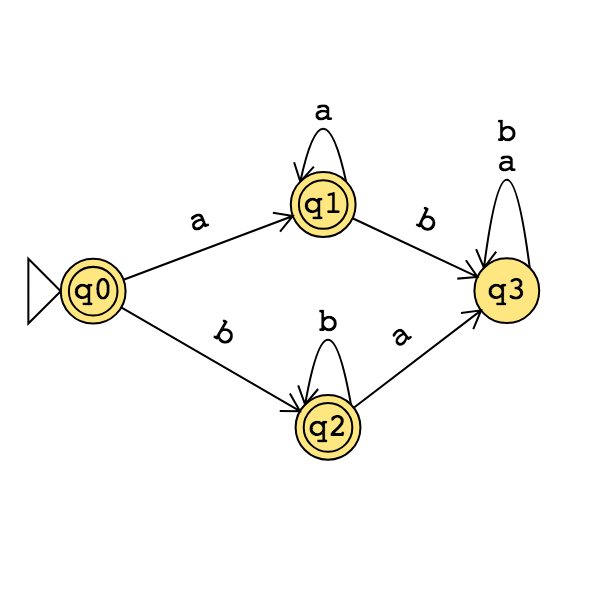
\includegraphics[width=2.5in]{../../resources/machines/Lect6NFA3.png}

\vfill
 \vfill
\section*{Week3 friday}


{\bf Definition and Theorem}: For an alphabet $\Sigma$, a language $L$ over $\Sigma$ is called {\bf regular}
exactly when $L$ is recognized by some DFA, which happens exactly when $L$ is recognized by some NFA, 
and happens exactly when $L$ is described by some regular expression

{\bf We saw that}: The class of regular languages is closed under complementation, union, 
intersection, set-wise concatenation, and Kleene star.

{\bf Prove or Disprove}: There is some alphabet $\Sigma$ for which there is 
some language recognized by an NFA but not by any DFA.

\vfill

{\bf Prove or Disprove}: There is some alphabet $\Sigma$ for which there is 
some finite language not described by any regular expression over $\Sigma$.

\vfill

{\bf Prove or Disprove}: If a language is recognized by an NFA 
then the complement of this language is not recognized by any DFA.

\vfill

\newpage

{\bf Fix alphabet $\Sigma$. Is every language $L$ over $\Sigma$ regular?}

\begin{center}
\begin{tabular}{c|c}
Set & Cardinality \\
\hline
& \\
$\{0,1\}$ & \\
& \\
$\{0,1\}^*$ & \\
& \\
$\mathcal{P}( \{0,1\})$ & \\
& \\
The set of all languages over $\{0,1\}$ & \\
& \\
The set of all regular expressions over $\{0,1\}$ & \\
& \\
The set of all regular languages over $\{0,1\}$ & \\
& \\
\end{tabular}
\end{center}



\vfill
Strategy: Find an {\bf invariant} property that is true of all regular languages. When analyzing 
a given language, if the invariant is not true about it, then the language is not regular.
\newpage

{\bf Pumping Lemma} (Sipser Theorem 1.70): If $A$ is a regular language, then there
is a number $p$ (a {\it pumping length}) where, if $s$ is any string in $A$ of length at least $p$, 
then $s$ may be divided into three pieces, $s = xyz$ such that
\vspace{-10pt}
\begin{itemize}
\item $|y| > 0$
\item for each $i \geq 0$, $xy^i z \in A$
\item $|xy| \leq p$.
\end{itemize}


{\bf Proof illustration}


\vfill




{\bf True or False}: A pumping length for $A = \{ 0,1 \}^*$ is $p = 5$.

\vspace{50pt} \vfill
\section*{Week2 wednesday}



{\bf Review}: Formal definition of finite automaton: $M = (Q, \Sigma, \delta, q_0, F)$ 

\begin{center}
\begin{multicols}{2}
\begin{itemize}
\setlength{\itemsep}{2pt}
\item Finite set of states $Q$
\item Alphabet $\Sigma$
\item Transition function $\delta$
\item Start state $q_0$
\item Accept (final) states $F$
\end{itemize}
\end{multicols}
\end{center}
In the state diagram of $M$, how many outgoing arrows are there from each state?

$M = ( \{ q, r, s\}, \{a,b\}, \delta, q, \{q\} )$ 
where $\delta$ is  (rows labelled by states
and columns labelled by symbols):
\begin{center}
\begin{tabular}{c|cc}
$\delta$ & $a$ & $b$ \\
\hline
$q$ & $r$ & $r$ \\
$r$ & $s$ & $s$ \\
$s$ & $q$ & $q$ \\
\end{tabular}
\end{center}

The state diagram for $M$ is 

\vfill



Give two examples of strings that are accepted by $M$ and two examples of strings that are rejected by $M$:

\vfill



$L(M) = $

A regular expression describing $L(M)$ is




\newpage
Let the alphabet be $\Sigma_1 = \{0,1\}$.

A state diagram for a finite automaton that recognizes $\{w \in \Sigma_1^* \mid w~\text{contains at most two $1$'s} \}$ is

\vfill

A state diagram for a finite automaton that recognizes $\{w \in \Sigma_1^* \mid w~\text{contains more than two $1$'s} \}$ is

\vfill

\textbf{Strategy}: Add ``labels" for states in the state diagram, e.g. 
``have not seen any of desired pattern yet'' or ``sink state''.
Then, we can use the analysis of the roles of the states in the state diagram to work towards a 
description of the language recognized by the finite automaton. 

\vfill
A useful bit of terminology: the {\bf iterated transition function} of a finite automaton
$M = (Q, \Sigma, \delta, q_0, F)$ is defined recursively by
\[
\delta^* (~(q,w)~) 
=\begin{cases}
q  \qquad &\text{if $q \in Q, w = \varepsilon$} \\
\delta( ~(q,a)~) \qquad &\text{if $q \in Q$, $w = a \in \Sigma$ } \\
\delta(~(\delta^*(q,u), a) ~) \qquad &\text{if $q \in Q$, $w = ua$ where $u \in  \Sigma^*$ and $a \in \Sigma$}
\end{cases}
\]

Using  this terminology, $M$ accepts a string $w$ over $\Sigma$ if and only if $\delta^*( ~(q_0,w)~) \in F$.

\newpage
Suppose $A$ is a language over an alphabet $\Sigma$. By definition, this means $A$ is a subset of $\Sigma^*$.
{\bf Claim:} if there is a DFA $M$ such that $L(M) = A$ then there is another DFA, let's call it $M'$, such that 
$L(M') = \overline{A}$, the complement of $A$, defined as $\{ w \in \Sigma^* \mid w \notin A \}$.

{\bf Proof idea}:


{\bf Proof}: 




\vfill

Application: Design a finite automaton that recognizes the language of all strings over $\{a,b\}$
whose length is not a multiple of $3$.

\vfill

{\bf Note}: On Friday, we'll see a new kind of finite automaton. It will be helpful to distinguish it from the
machines we've been talking about so we'll use {\bf Deterministic Finite Automaton} (DFA) to refer to the machines 
from Section 1.1. \vfill
\section*{Week2 friday}



\begin{center}
\begin{tabular}{|ll|}
\hline
\multicolumn{2}{|l|}{{\bf Nondeterministic finite automaton}  (Sipser Page 53) Given as $M = (Q, \Sigma, \delta, q_0, F)$}\\
& \\
Finite set of states $Q$  & Can  be labelled by any collection  of distinct names. Default: $q0, q1, \ldots$  \\
Alphabet $\Sigma$ &  Each input to the automaton is a string over  $\Sigma$. \\
Arrow labels $\Sigma_\varepsilon$ &  $\Sigma_\varepsilon = \Sigma \cup \{ \varepsilon\}$. \\
&  Arrows 
in the state diagram are labelled either by symbols from $\Sigma$ or by $\varepsilon$ \\
Transition function $\delta$  & $\delta: Q \times \Sigma_{\varepsilon} \to \mathcal{P}(Q)$
gives the {\bf set of possible next states} for a transition \\
&  from the current state upon reading a symbol or spontaneously moving.\\
Start state $q_0$ & Element of $Q$.  Each computation of the machine starts at the  start  state.\\
Accept (final) states $F$ & $F \subseteq  Q$.\\
& \\
\multicolumn{2}{|p{\textwidth}|}{$M$ accepts the input string $w \in \Sigma^*$ if and only if {\bf there is} a computation of $M$ on 
$w$ that processes the whole string and ends in an
accept state.}\\
\hline
\end{tabular}
\end{center}

The formal definition of the NFA over $\{0,1\}$ given by this state diagram is: 

\includegraphics[width=2in]{../../resources/machines/Lect4NFA1.png}

The language over $\{0,1\}$ recognized by this NFA is:

\vspace{70pt}

Change the transition function to get a different NFA which accepts
the empty string (and potentially other strings too).


\newpage

The state diagram of an NFA over $\{a,b\}$ is below.  The formal definition of this NFA is:

\vspace{-30pt}

\includegraphics[width=2.5in]{../../resources/machines/Lect5NFA1.png}


\vspace{-10pt}

The language recognized by this NFA is:  \vfill
\section*{Week1 monday}


The CSE 105 vocabulary and notation build on discrete
math and introduction to proofs classes.  Some of the conventions may 
be a bit different from what you saw before so we'll draw your attention to them.

For consistency, we will use the notation from this class' textbook\footnote{Page references are to 
the 3rd edition of Sipser's Introduction to the Theory of Computation,
available through various sources for approximately \$30. You may be able to 
opt in to purchase a digital copy through Canvas. Copies of the book are also available 
for those who can't access the book
to borrow from the course instructor, while supplies last (minnes@ucsd.edu)}.

These definitions are on pages 3, 4, 6, 13, 14, 53.

\begin{center}
    \begin{tabular}{|p{2.6in}cp{3.5in}|}
    \hline 
    {\bf Term} & {\bf Typical symbol} & {\bf Meaning} \\
     & or {\bf Notation} & \\
    \hline
    && \\
    Alphabet & $\Sigma$, $\Gamma$ & A non-empty finite set	 \\
    Symbol over $\Sigma$  & $\sigma$, $b$, $x$ & An element of the alphabet $\Sigma$\\ 
    String over $\Sigma$  &	$u$, $v$, $w$ & A finite list of symbols from $\Sigma$\\
    (The) empty string &$\varepsilon$ & The (only) string of length $0$\\
    The set of all strings over $\Sigma$ & $\Sigma^*$ & The collection of all possible strings formed from symbols from $\Sigma$ \\ 
    (Some) language over $\Sigma$& $L$ & (Some) set of strings over $\Sigma$ \\ 
    (The) empty language &$\emptyset$ & The empty set, i.e. the set that has no strings (and no other elements either)\\
    && \\
    \hline
    && \\
    The power set of a set $X$ &$\mathcal{P}(X)$ & The set of all subsets of $X$ \\
    (The set of) natural numbers &$\mathcal{N}$ & The set of positive integers \\ 
    (Some) finite set & & The empty set or a set whose distinct elements can be counted by a natural number\\
    (Some) infinite set & & A set that is not finite.\\ 
    &&\\
    \hline
    && \\
    Reverse of a string $w$ & $w^\mathcal{R}$  & write $w$  in  the opposite order, if $w = w_1 \cdots  w_n$ then $w^\mathcal{R} = w_n \cdots  w_1$. Note: $\varepsilon^\mathcal{R} = \varepsilon$\\
    Concatenating strings $x$ and $y$ & $xy$ &  take $x = x_1 \cdots x_m$, $y=y_1 \cdots y_n$ and form $xy = x_1 \cdots x_m y_1 \cdots y_n$\\
    String $z$ is a substring of string $w$ & & there are strings $u,v$ such that $w = uzv$\\
    String $x$ is a prefix of string $y$ & & there is a string $z$ such that $y = xz$ \\
    String $x$ is a proper prefix of string $y$ & & $x$ is a prefix of $y$ and $x \neq y$\\
    && \\
    \hline
    &&\\
    Shortlex order, also known as string order over alphabet $\Sigma$ & & Order strings over  $\Sigma$ first 
    by length and then according to the dictionary order, assuming symbols in $\Sigma$  have an ordering\\ \hline
    \end{tabular}
\end{center}

\vfill
    
\newpage
Write out in words the meaning of the symbols below: 

\[
    \{ a, b, c\}
\]

\phantom{The set whose elements are $a$, $b$, and $c$}

\[
    | \{a, b, a \} | = 2
\]

\phantom{The number of elements in the set $\{a,b,a\}$ is $2$.}

\[
    | aba | = 3
\]

\phantom{The length of the string $aba$ is $3$.}

\begin{comment}

\[
    (a, 3, 2, b, b)
\]

\phantom{The $5$-tuple whose first components is $a$, second component 
is $3$, third component is $2$, fourth component is $b$, and fifth component is $b$.}
\end{comment}

{\it Circle the correct choice}:

A {\bf string} over an alphabet $\Sigma$ is \underline{~~an element of $\Sigma^*$ ~~ OR ~~ a subset of $\Sigma^*$}.
    
A {\bf language} over an alphabet $\Sigma$ is \underline{~~an element of $\Sigma^*$ ~~ OR ~~ a subset of $\Sigma^*$}.


With $\Sigma_1 = \{0,1\}$ and 
$\Sigma_2 = \{a,b,c,d,e,f,g,h,i,j,k,l,m,n,o,p,q,r,s,t,u,v,w,x,y,z\}$
and $\Gamma = \{0,1,x,y,z\}$

{\bf True} or {\bf False}: $\varepsilon \in \Sigma_1$

{\bf True} or {\bf False}: $\varepsilon$ is  a string over $\Sigma_1$

{\bf True} or {\bf False}: $\varepsilon$ is a language over $\Sigma_1$

{\bf True} or {\bf False}: $\varepsilon$ is a prefix of some string over  $\Sigma_1$

{\bf True} or {\bf False}: There is a string over $\Sigma_1$ that is a proper prefix of $\varepsilon$
    

The first five strings over $\Sigma_1$ in string order, using the ordering $0 <  1$: \vfill
    
The first five strings over $\Sigma_2$ in string order, using the usual alphabetical ordering for single letters: \vfill



 \vfill
\section*{Week1 wednesday}


Our motivation in studying sets of strings is that they can be used to encode problems.
To calibrate how difficult a problem is to solve, we describe how complicated the set of strings that encodes it is. 
How do we define sets of strings?


\vfill

How would you describe the language that has no elements at all?

\vfill

How would you describe the language that has all strings over $\{0,1\}$ as its elements?

\vfill

\newpage

**This definition was in the pre-class reading**
{\bf Definition 1.52}: A {\bf regular expression} over alphabet $\Sigma$
is a syntactic expression that can describe a language over $\Sigma$. The collection of all regular
expressions over $\Sigma$ is defined recursively:
\begin{itemize}
\item[] {\it Basis steps of recursive definition}
\begin{quote}    
    $a$ is a regular expression, for $a \in \Sigma$

    $\varepsilon$ is a regular expression

    $\emptyset$ is a regular expression
\end{quote}

\item[] {\it Recursive steps of recursive definition}
\begin{quote}
    $(R_1 \cup R_2)$ is a regular expression when $R_1$, $R_2$ are regular expressions 

    $(R_1 \circ R_2)$ is a regular expression when $R_1$, $R_2$ are regular expressions

    $(R_1^*)$ is a regular expression when $R_1$ is a regular expression 
\end{quote}
\end{itemize}
 

The {\it semantics} (or meaning) of the syntactic regular expression is the {\bf language
described by the regular expression}. The function that assigns a language to a regular expression
over $\Sigma$ is defined recursively, using familiar set operations:


\begin{itemize}
    \item[] {\it Basis steps of recursive definition}
    \begin{quote}    
        The language described by $a$, for $a \in \Sigma$, is $\{a\}$ and we write 
        $L(a) = \{a\}$
    
        The language described by $\varepsilon$ is $\{\varepsilon\}$ and we write 
        $L(\varepsilon) = \{ \varepsilon\}$
    
        The language described by $\emptyset$ is $\{\}$ and we write
        $L(\emptyset) = \emptyset$.
    \end{quote}
    
    \item[] {\it Recursive steps of recursive definition}
    \begin{quote}
        When $R_1$, $R_2$ are regular expressions, the language described by the regular
        expression $(R_1 \cup R_2)$ is the union of the languages described by $R_1$ and $R_2$, 
        and we write 
        $$L(~(R_1 \cup R_2)~) = L(R_1) \cup L(R_2) = \{ w \mid w \in L(R_1) \lor w \in L(R_2)\}$$
    
        When $R_1$, $R_2$ are regular expressions, the language described by the regular
        expression $(R_1 \circ R_2)$ is the concatenation of the languages described by $R_1$ and $R_2$, 
        and we write 
        $$L(~(R_1 \circ R_2)~) = L(R_1) \circ L(R_2) = \{ uv \mid u \in L(R_1) \land v \in L(R_2)\}$$
    
        When $R_1$ is a regular expression, the language described by the regular 
        expression $(R_1^*)$ is the {\bf Kleene star} of the language described by $R_1$ and we write
        $$L(~(R_1^*)~) = (~L(R_1)~)^* = \{ w_1 \cdots w_k \mid k \geq 0 \textrm{ and each } w_i \in L(R_1)\}$$
    \end{quote}
\end{itemize}
  
\newpage
For the following examples assume the alphabet is $\Sigma_1 =  \{0,1\}$:
    
The language described by the regular expression $0$ is $L(0) = \{ 0 \}$

The language described by the regular expression $1$ is $L(1)  = \{ 1 \}$

The language described by the regular expression $\varepsilon$ is $L(\varepsilon) = \{ \varepsilon  \}$

The language described by the regular expression $\emptyset$ is $L(\emptyset) = \emptyset$

The language described by the regular expression $(\Sigma_1 \Sigma_1 \Sigma_1)^*$ 
is $L(~(\Sigma_1 \Sigma_1 \Sigma_1)^*~) = $

\vfill

The language described by the regular expression $1^+$ is $L(~(1^+)~) = L(1^* \circ 1) = $

\vfill


{\it Shorthand and conventions} (Sipser pages 63-65)
\begin{center}
    \begin{tabular}{|ll|}
    \hline
    & \\
    \multicolumn{2}{|l|}{Assuming $\Sigma$ is the alphabet, we use the following conventions}\\
    & \\
    $\Sigma$   & regular  expression describing language consisting of  all strings  of length  $1$ over $\Sigma$\\
    $*$ then $\circ$ then $\cup$   & precedence order, unless parentheses are used to change it\\
    $R_1R_2$ & shorthand  for  $R_1  \circ R_2$ (concatenation symbol is implicit) \\
    $R^+$ & shorthand for $R^* \circ R$ \\
    $R^k$ & shorthand for $R$ concatenated with itself $k$ times, where $k$ is a (specific) natural number\\
    & \\
    \hline
    \end{tabular}
\end{center}

\newpage
{\bf Caution: many programming languages that support regular expressions build in functionality
that is more powerful than the ``pure'' definition of regular expressions given here. }

Regular expressions are everywhere (once you start looking for them).

Software tools and languages often have built-in support for regular expressions to describe
{\bf patterns} that we want to match (e.g. Excel/ Sheets, grep, Perl, python, Java, Ruby).

Under the hood, the first phase of {\bf compilers} is to transform the strings we write 
in code to tokens (keywords, operators, identifiers, literals). Compilers use regular expressions
to describe the sets of strings that can be used for each token type.

Next time: we'll start to see how to build machines that decide whether strings match the pattern
described by a regular expression.

\vfill


{\it Extra examples for practice:}

Which regular expression(s) below describe a language that includes the string $a$ as an element?

$a^* b^*$ 

\vfill

$a(ba)^* b$

\vfill

$a^* \cup b^*$

\vfill

$(aaa)^*$

\vfill

$(\varepsilon \cup a) b$

\vfill \vfill
\section*{Week1 friday}


{\bf Review}: Determine whether each statement below about regular expressions
over the alphabet $\{a,b,c\}$ is true or false:

\begin{comment}
True or False: \qquad 
   $a  \in L(~(a \cup b )~\cup c)$
\end{comment}

True or False: \qquad 
   $ab  \in L(~ (a \cup b)^*  ~)$
   
True or False: \qquad    
   $ba \in L( ~ a^* b^* ~)$
   
True or False: \qquad 
   $\varepsilon  \in L(a \cup b \cup c)$
   
True or False: \qquad 
   $\varepsilon  \in L(~ (a \cup b)^*  ~)$

True or False: \qquad 
   $\varepsilon \in L( ~ aa^* \cup bb^* ~)$


**This definition was in the pre-class reading**
A finite automaton (FA) is specified by  $M = (Q, \Sigma, \delta, q_0, F)$.
This $5$-tuple is called the {\bf formal definition} of the FA. The FA can also 
be represented by its state diagram: with nodes for the state, labelled edges specifying the 
transition function, and decorations on nodes denoting the start and accept states.

\begin{quote}
Finite set of states $Q$ can be labelled by any collection of distinct names. Often
we use default state labels $q0, q1, \ldots$ 
\end{quote}

\begin{quote}  
The alphabet $\Sigma$ determines the possible inputs to the automaton. 
Each input to the automaton is a string over  $\Sigma$, and the automaton ``processes'' the input
one symbol (or character) at a time.
\end{quote}

\begin{quote}
The transition function $\delta$ gives the next state of the automaton based on the current state of 
the machine and on the next input symbol.
\end{quote}

\begin{quote}
The start state $q_0$ is an element of $Q$.  Each computation of the machine starts at the  start  state.
\end{quote}

\begin{quote}
The accept (final) states $F$ form a subset of the states of the automaton, $F \subseteq  Q$. 
These states are used to flag if the machine accepts or rejects an input string.
\end{quote}


\begin{quote}
The computation of a machine on an input string is a sequence of states
in the machine,  starting with the start state, determined by transitions 
of the machine as it reads successive input symbols.
\end{quote}

\begin{quote}
The finite automaton $M$ accepts the given input string exactly when the computation of $M$ on the input string
ends in an accept state. $M$ rejects the given input string exactly when the computation of 
$M$ on the input string ends in a nonaccept state, that is, a state that is not in $F$.
\end{quote}

\begin{quote} 
The language of $M$, $L(M)$, is defined as the set of  all strings that are each accepted 
by the machine $M$. Each string that is rejected by $M$ is not in $L(M)$.
The language of $M$ is also called the language recognized by $M$.
\end{quote}   
   
What is {\bf finite} about all finite automata? (Select all that apply)
\begin{itemize}
   \item[$\square$] The size of the machine (number of states, number of arrows)
   \item[$\square$] The length of each computation of the machine
   \item[$\square$] The number of strings that are accepted by the machine
\end{itemize}
  
\begin{figure}[h]
   \centering
   \includegraphics[width=3in]{../../resources/machines/Lect2DFA1.png} 
\end{figure}
   
The formal definition of this FA is
   
\vspace{100pt}
   

Classify each string $a, aa, ab, ba, bb, \varepsilon$ as accepted by the FA or rejected by the FA.  

{\it Why are these the only two options?}

\vspace{200pt}


The language recognized by this automaton is
  
\vspace{100pt}
   

\begin{figure}[h]
  \centering
  \includegraphics[width=3in]{../../resources/machines/Lect2DFA2.png} 
\end{figure}
   

The language recognized by this automaton is
  
\vspace{100pt}

\begin{figure}[h]
    \centering
    \includegraphics[width=3in]{../../resources/machines/Lect2DFA3.png} 
\end{figure}

The language recognized by this automaton is
  
\vspace{100pt}
 \vfill
\section*{Week10 friday}


\begin{center}
    \begin{tabular}{|p{4in}|p{3.5in}|}
        \hline
        & \\
        {\bf Model of Computation} & {\bf Class of Languages}\\
        &\\
        \hline
        & \\
        {\bf Deterministic finite automata}:
        formal definition, how to design for a given language, 
        how to describe language of a machine?
        {\bf Nondeterministic finite automata}:
        formal definition, how to design for a given language, 
        how to describe language of a machine?
        {\bf Regular expressions}: formal definition, how to design for a given language, 
        how to describe language of expression?
        {\it Also}: converting between different models. &
        {\bf Class of regular languages}: what are the closure 
        properties of this class? which languages are not in the class?
        using {\bf pumping lemma} to prove nonregularity.\\
        & \\
        \hline
        & \\
        {\bf Push-down automata}:
        formal definition, how to design for a given language, 
        how to describe language of a machine?
        {\bf Context-free grammars}:
        formal definition, how to design for a given language, 
        how to describe language of a grammar? &
        {\bf Class of context-free languages}: what are the closure 
        properties of this class? which languages are not in the class?\\
        & \\
        \hline
        & \\
        Turing machines that always halt in polynomial time
        & $P$ \\
        & \\
        Nondeterministic Turing machines that always halt in polynomial time 
        & $NP$ \\
        & \\
        \hline
        & \\
        {\bf Deciders} (Turing machines that always halt): 
        formal definition, how to design for a given language, 
        how to describe language of a machine? &
        {\bf Class of decidable languages}: what are the closure properties 
        of this class? which languages are not in the class? using diagonalization
        and mapping reduction to show undecidability \\
        & \\
        \hline
        & \\
        {\bf Turing machines}
        formal definition, how to design for a given language, 
        how to describe language of a machine? &
        {\bf Class of recognizable languages}: what are the closure properties 
        of this class? which languages are not in the class? using closure
        and mapping reduction to show unrecognizability \\
        & \\
        \hline
    \end{tabular}
\end{center}

\newpage

{\bf Given a language, prove it is regular}

{\it Strategy 1}: construct DFA recognizing the language and prove it works.

{\it Strategy 2}: construct NFA recognizing the language and prove it works.

{\it Strategy 3}: construct regular expression recognizing the language and prove it works.

{\it ``Prove it works'' means \ldots}

\vspace{100pt}

{\bf Example}: $L  = \{ w \in \{0,1\}^* \mid \textrm{$w$ has odd number of $1$s or starts with $0$}\}$

Using NFA

\vfill

Using regular expressions

\vfill


\newpage

{\bf Example}: Select all and only the options that result in a true statement: ``To show 
a language $A$ is not regular, we can\ldots'' 

\begin{enumerate}
    \item[a.] Show $A$ is finite
    \item[b.] Show there is a CFG generating $A$
    \item[c.] Show $A$ has no pumping length
    \item[d.] Show $A$ is undecidable
\end{enumerate}

\newpage

{\bf Example}: What is the language generated by the CFG with rules
\begin{align*}
    S &\to aSb \mid bY \mid Ya \\
    Y &\to bY \mid Ya \mid \varepsilon 
\end{align*}

\newpage

{\bf Example}: Prove that the language 
$T = \{ \langle M \rangle \mid \textrm{$M$ is a Turing machine and $L(M)$ is infinite}\}$ 
is undecidable.

\newpage

{\bf Example}: Prove that the class of decidable languages is closed under concatenation.
 \vfill
\end{document}